\chapter{Valores y vectores propios}\label{vvpropios}
En este capítulo se estudian los valores y vectores propios de una matriz cuadrada $A$: los vectores no nulos que la matriz no ``tuerce'', sino que únicamente estira, contrae o invierte, de modo que $A\mathbf{v}=\lambda\mathbf{v}$ para algún escalar $\lambda$. Hallarlos se reduce a resolver la ecuación característica $\det(\lambda I-A)=0$, un polinomio en $\lambda$ que conecta este capítulo con las técnicas de determinantes del Capítulo~\ref{matrdet}, mientras que el espacio propio asociado a cada $\lambda$ se calcula como el espacio nulo de la matriz $\lambda I-A$ con los métodos del Capítulo~\ref{sel}. Sobre estos conceptos se construye la diagonalización $A=PDP^{-1}$, que permite calcular potencias $A^{k}$ de manera eficiente y resolver sistemas de ecuaciones diferenciales lineales; este último tema se retoma de forma sistemática en el Capítulo~\ref{sistemasedos}. El capítulo cierra con el teorema de Cayley-Hamilton y una muestra de aplicaciones adicionales: cadenas de Markov, formas cuadráticas y sistemas dinámicos.

\section{Valores y vectores propios}

\begin{definition}[Valores y vectores propios]
	Sea $A$ una matriz cuadrada $n\times n$. Un vector no nulo $\mathbf{v}\in \mathbb{R}^n$ es llamado \textbf{vector propio} (también conocido como \textbf{autovector} o \textbf{eigenvector}) de la matriz $A$ asociado al \textbf{valor propio} $\lambda \in \mathbb{R}$ (también llamado \textbf{autovalor} o \textbf{eigenvalor}) si satisface la ecuación:
	$$\boxed{A\mathbf{v} = \lambda \mathbf{v}}$$
	
	Reescribiendo esta ecuación, obtenemos: $\mathbf{0} = A\mathbf{v} - \lambda \mathbf{v} = (A - \lambda I_n)\mathbf{v}.$
	
	Para que existan vectores propios no nulos $\mathbf{v}$, la matriz $(A - \lambda I_n)$ debe ser singular, es decir:
	$$\det(A - \lambda I_n) = 0$$
	
	Esta ecuación es conocida como la \textbf{ecuación característica de la matriz $A$}. Sus soluciones $\lambda$ son los valores propios de $A$.
	
	Para cada valor propio $\lambda_i$, los vectores propios correspondientes forman el espacio nulo de la matriz $(A - \lambda_i I_n)$, es decir: $E_{\lambda_i} = \ker(A - \lambda_i I_n) = \{\mathbf{v} \in \mathbb{R}^n : (A - \lambda_i I_n)\mathbf{v} = \mathbf{0}\}.$
\end{definition}

\begin{figure}[H]
\centering
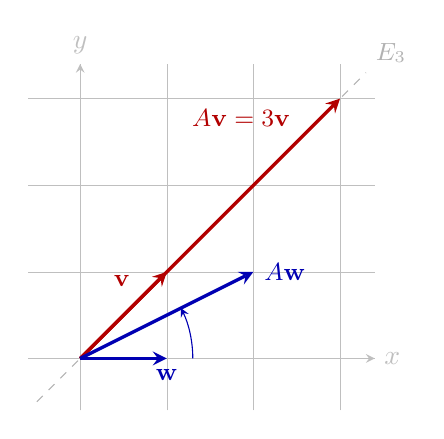
\begin{tikzpicture}[scale=1.1, >=stealth]
\draw[gray!50, very thin] (-0.6,-0.6) grid (3.4,3.4);
\draw[->, gray!50] (-0.6,0) -- (3.4,0) node[anchor=west] {$x$};
\draw[->, gray!50] (0,-0.6) -- (0,3.4) node[anchor=south] {$y$};
% Dirección propia (recta y = x)
\draw[dashed, gray!60] (-0.5,-0.5) -- (3.3,3.3) node[anchor=south west] {\small $E_{3}$};
% Vector propio v y su imagen Av = 3v (misma dirección)
\draw[->, red!70!black, very thick] (0,0) -- (3,3) node[pos=0.85, above left] {\small $A\mathbf{v}=3\mathbf{v}$};
\draw[->, red!70!black, very thick] (0,0) -- (1,1) node[pos=0.7, above left] {\small $\mathbf{v}$};
% Vector genérico w y su imagen Aw (cambia de dirección)
\draw[->, blue!70!black, very thick] (0,0) -- (1,0) node[below] {\small $\mathbf{w}$};
\draw[->, blue!70!black, very thick] (0,0) -- (2,1) node[anchor=west] {\small $A\mathbf{w}$};
% Arco que indica el giro de w hacia Aw
\draw[->, blue!70!black] (1.3,0) arc[start angle=0, end angle=26.6, radius=1.3];
\end{tikzpicture}
\caption{Acción de la matriz $A=\left(\begin{smallmatrix}2&1\\1&2\end{smallmatrix}\right)$ sobre dos vectores. El vector propio $\mathbf{v}=(1,1)$ no cambia de dirección: solo se estira, $A\mathbf{v}=3\mathbf{v}$, y su recta $E_{3}$ queda invariante. En cambio, el vector genérico $\mathbf{w}=(1,0)$ sí gira: $A\mathbf{w}=(2,1)$ no es múltiplo de $\mathbf{w}$.}
\label{fig:accion_vector_propio}
\end{figure}

\begin{example}[Valores propios de una matriz $2\times2$]\label{ex:ejemplovvp}
	Sea $A = \begin{pmatrix} 1 & 2 \\ 3 & 2 \end{pmatrix}$. Calcule sus valores propios.
	\begin{myproof}
	\textbf{Paso 1.} Planteamos la ecuación característica $\det(\lambda I - A)=0$:
	\[
	\det\begin{pmatrix} \lambda - 1 & -2 \\ -3 & \lambda - 2 \end{pmatrix} = 0 \quad\Rightarrow\quad (\lambda-1)(\lambda-2)-(-2)(-3)=\lambda^2-3\lambda-4=0.
	\]

	\textbf{Paso 2.} Resolvemos la ecuación cuadrática:
	\[
	\lambda = \frac{3 \pm \sqrt{9+16}}{2} = \frac{3 \pm 5}{2} \quad\Rightarrow\quad \lambda_1 = 4, \quad \lambda_2 = -1.
	\]

	\textbf{Paso 3.} Los valores propios de $A$ son $\boxed{\lambda_1=4 \text{ y } \lambda_2=-1}$.
\end{myproof}

\end{example}

Según el teorema fundamental del álgebra (Teorema \ref{tfam}), todo polinomio no constante de grado $n$ con coeficientes complejos tiene exactamente $n$ raíces complejas contando multiplicidades. En el contexto del álgebra lineal, los valores $\lambda$ que son raíces del polinomio característico de $A$ se denominan \textbf{valores propios} de $A$.

\begin{definition}[Multiplicidad algebraica y geométrica]\label{multiplicidadgeometrica}
Para cada valor propio $\lambda$ de una matriz $A$, se definen:
\begin{itemize}
    \item \textbf{Multiplicidad algebraica}: Número de veces que $\lambda$ aparece como raíz del polinomio característico $\det(\lambda I - A) = 0$.
    \item \textbf{Multiplicidad geométrica}: Dimensión del espacio propio asociado a $\lambda$, es decir: \(\dim \ker(\lambda I - A).\)
\end{itemize}
\end{definition}

\begin{rem}
En el ejemplo \ref{ex:ejemplovvp} con $A = \begin{pmatrix} 1 & 2 \\ 3 & 2 \end{pmatrix}$, ambos valores propios ($\lambda = -1$ y $\lambda = 4$) tienen multiplicidad algebraica 1 y geométrica 1. 

Considere ahora la matriz $B = \begin{pmatrix} a & 0 \\ 0 & a \end{pmatrix}$. Su polinomio característico es \[
\det(\lambda I - B) = \det\begin{pmatrix} \lambda - a & 0 \\ 0 & \lambda - a \end{pmatrix} = (\lambda - a)^2 \], la única raíz es $\lambda = a$ con multiplicidad algebraica 2 y su multiplicidad geométrica también es 2, pues \(
\ker(aI - B) = \ker\begin{pmatrix} 0 & 0 \\ 0 & 0 \end{pmatrix} = \mathbb{R}^2
\) que tiene dimensión 2.
\end{rem}


\begin{theorem}[Caracterización de valores propios]\label{teo:caracterizacion}
Sea $A \in M_n(\mathbb{R})$. Las siguientes afirmaciones son equivalentes:
\begin{enumerate}[$(1)$]
    \item $\lambda$ es un valor propio de $A$.
    \item $\lambda$ es solución de la ecuación característica $\det(\lambda I - A) = 0$.
    \item Existe un vector no nulo $\mathbf{x} \in \mathbb{R}^n$ tal que $A\mathbf{x} = \lambda \mathbf{x}$.
\end{enumerate}
\end{theorem}

\begin{proof}
Demostramos las equivalencias:

\textbf{$(1)$) $\Rightarrow$ ($(3)$)}: Por definición de valor propio, existe $\mathbf{x} \neq \mathbf{0}$ tal que $A\mathbf{x} = \lambda\mathbf{x}$.

\textbf{$(3)$ $\Rightarrow$ ($(2)$)}: Si $A\mathbf{x} = \lambda\mathbf{x}$, entonces $(\lambda I - A)\mathbf{x} = \mathbf{0}$. Como $\mathbf{x} \neq \mathbf{0}$, la matriz $\lambda I - A$ es singular, luego $\det(\lambda I - A) = 0$.

\textbf{$(2)$ $\Rightarrow$ $(1)$}: Si $\det(\lambda I - A) = 0$, entonces $\lambda I - A$ es singular y existe $\mathbf{x} \neq \mathbf{0}$ tal que $(\lambda I - A)\mathbf{x} = \mathbf{0}$, es decir, $A\mathbf{x} = \lambda\mathbf{x}$.
\end{proof}

\begin{coro}[Valores propios de matrices triangulares]\label{cor:triangular}
Si $A$ es una matriz triangular, sus valores propios son los elementos de su diagonal principal.
\end{coro}

\begin{proof}
Para una matriz triangular $A = (a_{ij})$, el polinomio característico es:
\[
\det(\lambda I - A) = \prod_{i=1}^n (\lambda - a_{ii})
\]
Las raíces son $\lambda_i = a_{ii}$ para $i=1,\dots,n$.
\end{proof}

\begin{coro}[Invertibilidad y el valor propio cero]\label{cor:cerovp}
Una matriz $A\in M_n(\mathbb{R})$ es invertible si y solo si $\lambda=0$ no es un valor propio de $A$.
\end{coro}

\begin{proof}
Por el Teorema \ref{teo:caracterizacion}:
\[
\det(A) = 0 \iff \det(0 \cdot I - A) = 0 \iff \lambda = 0 \text{ es valor propio}
\]
Como $A$ es invertible si y solo si $\det(A) \neq 0$, el resultado sigue.
\end{proof}

\begin{theorem}[Potencia de valores propios]\label{teo:potencia}
Si $\lambda$ es valor propio de $A \in M_n(\mathbb{R})$ con vector propio asociado $\mathbf{x}$, entonces para todo $k \in \mathbb{Z}^+$, $\lambda^k$ es valor propio de $A^k$ con el mismo vector propio $\mathbf{x}$.
\end{theorem}

\begin{proof}
Por inducción sobre $k$:

\textbf{Caso base} ($k=1$): Por hipótesis, $A\mathbf{x} = \lambda\mathbf{x}$.

\textbf{Paso inductivo}: Supongamos $A^k\mathbf{x} = \lambda^k\mathbf{x}$. Entonces:
\[
A^{k+1}\mathbf{x} = A(A^k\mathbf{x}) = A(\lambda^k\mathbf{x}) = \lambda^k(A\mathbf{x}) = \lambda^k(\lambda\mathbf{x}) = \lambda^{k+1}\mathbf{x}
\]
Por inducción, el resultado vale para todo $k \in \mathbb{Z}^+$.
\end{proof}

\begin{example}[Aplicación del teorema de potencias]
Sea $A$ una matriz con valor propio $\lambda_1 = 3$ y vector propio asociado $\mathbf{x} = \begin{pmatrix} 1 \\ 1 \\ 1 \end{pmatrix}$. Por el Teorema \ref{teo:potencia}, $A^5$ tiene valor propio $\lambda_1^5 = 3^5 = 243$ con el mismo vector propio $\mathbf{x}$.
\end{example}


\begin{example}[Valores y vectores propios y sus multiplicidades]\label{ex:vvp_multiplicidades} Dadas las siguientes matrices calcule sus valores y vectores propios, determine las multiplicidades algebraicas y geométricas correspondientes a cada valor propio.
  \begin{enumerate}[$a)$]
  \item $A=\left( \begin{array}{ccc} 
	1&2&2 \\
	0&2&1\\
	-1&2&2\\
	\end{array} \right).$ 
\begin{myproof}
\textbf{Paso 1.} Calculamos el polinomio característico: \(
\det(\lambda I - A) = \det\begin{pmatrix}
\lambda-1 & -2 & -2 \\
0 & \lambda-2 & -1 \\
1 & -2 & \lambda-2
\end{pmatrix}
\)

Aplicamos operaciones elementales:
\begin{align*}
& \xrightarrow{f_3 + f_1 \to f_3} \det\begin{pmatrix}
\lambda-1 & -2 & -2 \\
0 & \lambda-2 & -1 \\
\lambda & -4 & \lambda-4
\end{pmatrix} \\
& \xrightarrow{f_3 - \lambda f_2 \to f_3} \det\begin{pmatrix}
\lambda-1 & -2 & -2 \\
0 & \lambda-2 & -1 \\
0 & -4 + \lambda(2-\lambda) & \lambda-4 + \lambda
\end{pmatrix}
\end{align*}

Desarrollando por cofactores:
\[
= (\lambda-1)\left[(\lambda-2)^2 - 2\right] + 2\left[0 + 1\right] - 2\left[0 - (\lambda-2)\right] = \lambda^3 - 5\lambda^2 + 8\lambda - 4
\]

\textbf{Paso 2.} Las raíces son $\lambda = 1$ (multiplicidad algebraica 1) y $\lambda = 2$ (multiplicidad algebraica 2).

\textbf{Paso 3.} Calculamos los espacios propios.

\textbf{Eigenvalor $\lambda=1$}:
\[
( I - A) = \begin{pmatrix}
0 & -2 & -2 \\
0 & -1 & -1 \\
1 & -2 & -1
\end{pmatrix} \xrightarrow{\text{forma escalonada}} \begin{pmatrix}
1 & -2 & -1 \\
0 & 1 & 1 \\
0 & 0 & 0
\end{pmatrix}
\]
Solución: $v_1 = \begin{pmatrix} -1 \\ -1 \\ 1 \end{pmatrix}$ (multiplicidad geométrica 1).

\textbf{Eigenvalor $\lambda=2$}:
\[
(2I - A) = \begin{pmatrix}
1 & -2 & -2 \\
0 & 0 & -1 \\
1 & -2 & 0
\end{pmatrix} \xrightarrow{f_3 - f_1 \to f_3} \begin{pmatrix}
1 & -2 & -2 \\
0 & 0 & -1 \\
0 & 0 & 2
\end{pmatrix} \xrightarrow{f_3 + 2f_2 \to f_3} \begin{pmatrix}
1 & -2 & 0 \\
0 & 0 & 1 \\
0 & 0 & 0
\end{pmatrix}
\]
De $f_2$: $z = 0$. De $f_1$: $x = 2y$ (variable libre $y$).
Solución: $v_2 = \begin{pmatrix} 2 \\ 1 \\ 0 \end{pmatrix}$ (multiplicidad geométrica 1).

\textbf{Paso 4.} En resumen:
\[
\boxed{\lambda=1\ (\text{m.a.}=\text{m.g.}=1), \qquad \lambda=2\ (\text{m.a.}=2,\ \text{m.g.}=1).}
\]
Como la multiplicidad algebraica de $\lambda=2$ es $2$ pero la geométrica es $1$, la matriz $A$ \textbf{no es diagonalizable} (se requiere la forma canónica de Jordan para su representación canónica; véase la Subsección \ref{subsec:jordan}).
\end{myproof}
	
	\item $A=\left( \begin{array}{ccc} 
	1&2&4 \\
	0&2&3\\
	0&0&5\\
	\end{array} \right).$ 
\begin{myproof}
\textbf{Paso 1.} La matriz es triangular superior; por el Corolario \ref{cor:triangular} sus valores propios son los elementos de la diagonal:
$\lambda_1 = 1$ (mult. alg. 1), $\lambda_2 = 2$ (mult. alg. 1), $\lambda_3 = 5$ (mult. alg. 1).

\textbf{Paso 2.} Calculamos los espacios propios.

\textbf{Eigenvalor $\lambda=1$}:
\[
(I - A) = \begin{pmatrix}
0 & -2 & -4 \\
0 & -1 & -3 \\
0 & 0 & -4
\end{pmatrix} \xrightarrow{\text{forma escalonada}} \begin{pmatrix}
0 & 1 & 0 \\
0 & 0 & 1 \\
0 & 0 & 0
\end{pmatrix}
\]
Solución: $v_1 = \begin{pmatrix} 1 \\ 0 \\ 0 \end{pmatrix}$ (mult. geom. 1).

\textbf{Eigenvalor $\lambda=2$}:
\[
(2I - A) = \begin{pmatrix}
1 & -2 & -4 \\
0 & 0 & -3 \\
0 & 0 & -3
\end{pmatrix} \xrightarrow{f_3 - f_2 \to f_3} \begin{pmatrix}
1 & -2 & -4 \\
0 & 0 & -3 \\
0 & 0 & 0
\end{pmatrix}
\]
Solución: $v_2 = \begin{pmatrix} 2 \\ 1 \\ 0 \end{pmatrix}$ (mult. geom. 1).

\textbf{Eigenvalor $\lambda=5$}:
\[
(5I - A) = \begin{pmatrix}
4 & -2 & -4 \\
0 & 3 & -3 \\
0 & 0 & 0
\end{pmatrix} \xrightarrow{f_2/3 \to f_2} \begin{pmatrix}
4 & -2 & -4 \\
0 & 1 & -1 \\
0 & 0 & 0
\end{pmatrix}
\]
Solución: $v_3 = \begin{pmatrix} 3/2 \\ 1 \\ 1 \end{pmatrix}$ (mult. geom. 1).

\textbf{Paso 3.} En resumen:
\[
\boxed{\lambda=1,\ \lambda=2\ \text{y}\ \lambda=5,\ \text{cada uno con m.a.}=\text{m.g.}=1.}
\]
\end{myproof}
	
	\item $A=\left(\begin{matrix}
-10 & -71 & -19 \\
3 & 34 & 9 \\
-1 & -61 & -16
\end{matrix}\right)$ 
\begin{myproof}
\textbf{Paso 1.} Polinomio característico: $\det(\lambda I - A) = \lambda^3 - 8\lambda^2 + 19\lambda - 12 = 0$.

\textbf{Paso 2.} Raíces: $\lambda_1=1$, $\lambda_2=3$, $\lambda_3=4$ (mult. alg. 1 cada una).

\textbf{Paso 3.} Calculamos los espacios propios.

\textbf{Eigenvalor $\lambda=1$}:
\[
(I - A) = \begin{pmatrix}
11 & 71 & 19 \\
-3 & -33 & -9 \\
1 & 61 & 17
\end{pmatrix} \xrightarrow{\text{reducción}} \begin{pmatrix}
1 & 0 & \frac{-2}{25} \\
0 & 1 & \frac{7}{25} \\
0 & 0& 0
\end{pmatrix} \to \cdots
\]
Solución: $v_1 = \begin{pmatrix} 2/25 \\ -7/25 \\ 1 \end{pmatrix}$ (mult. geom. 1).

\textbf{Eigenvalor $\lambda=3$}:
\[
(3I - A) = \begin{pmatrix}
13 & 71 & 19 \\
-3 & -31 & -9 \\
1 & 61 & 19
\end{pmatrix} \xrightarrow{\text{reducción}} \begin{pmatrix}
1 & 0 & 5/19 \\
0 & 1 & -6/19 \\
0 & 0 & 0
\end{pmatrix}
\]
Solución: $v_2 = \begin{pmatrix} 5/19 \\ -6/19 \\ 1 \end{pmatrix}$ (mult. geom. 1).

\textbf{Eigenvalor $\lambda=4$}:
\[
(4I - A) = \begin{pmatrix}
14 & 71 & 19 \\
-3 & -30 & -9 \\
1 & 61 & 20
\end{pmatrix} \xrightarrow{\text{reducción}} \begin{pmatrix}
1 & 0 & 1/3 \\
0 & 1 & -1/3 \\
0 & 0 & 0
\end{pmatrix}
\]
Solución: $v_3 = \begin{pmatrix} 1/3 \\ -1/3 \\ 1 \end{pmatrix}$ (mult. geom. 1).

\textbf{Paso 4.} En resumen:
\[
\boxed{\lambda=1,\ \lambda=3\ \text{y}\ \lambda=4,\ \text{cada uno con m.a.}=\text{m.g.}=1.}
\]
\end{myproof}

\item $A=\left(\begin{matrix}
4 & 1 & 0 & 1 \\
2 & 3 & 0 & 1 \\
-2 & 1 & 2 & -3 \\
2 & -1 & 0 & 5
\end{matrix}\right)$
\begin{myproof}
\textbf{Paso 1.} Polinomio característico: $(\lambda-2)^2(\lambda-4)(\lambda-6)=0$.

\textbf{Paso 2.} Eigenvalores: $\lambda_1=2$ (mult. alg. 2), $\lambda_2=4$ (mult. alg. 1), $\lambda_3=6$ (mult. alg. 1).

\textbf{Paso 3.} Calculamos los espacios propios.

\textbf{Eigenvalor $\lambda=2$}:
\[
(2I - A) = \begin{pmatrix}
-2 & -1 & 0 & -1 \\
-2 & -1 & 0 & -1 \\
2 & -1 & 0 & 3 \\
-2 & 1 & 0 & -3
\end{pmatrix} \xrightarrow{\text{reducción}} \begin{pmatrix}
1 & 0 & 0 & 1 \\
0 & 1 & 0 & -1 \\
0 & 0 & 0 & 0 \\
0 & 0 & 0 & 0
\end{pmatrix}
\]
Solución: $v_1 = \begin{pmatrix} -1 \\ 1 \\ 0 \\ 1 \end{pmatrix}, v_2 = \begin{pmatrix} 0 \\ 0 \\ 1 \\ 0 \end{pmatrix}$ (mult. geom. 2).

\textbf{Eigenvalor $\lambda=4$}:
\[
(4I - A) = \begin{pmatrix}
0 & -1 & 0 & -1 \\
-2 & 1 & 0 & -1 \\
2 & -1 & 2 & 3 \\
-2 & 1 & 0 & -1
\end{pmatrix} \xrightarrow{\text{reducción}} \begin{pmatrix}
1 & 0 & 0 & 1 \\
0 & 1 & 0 & 1 \\
0 & 0 & 1 & 1 \\
0 & 0 & 0 & 0
\end{pmatrix}
\]
Solución: $v_3 = \begin{pmatrix} -1 \\ -1 \\ -1 \\ 1 \end{pmatrix}$ (mult. geom. 1).

\textbf{Eigenvalor $\lambda=6$}:
\[
(6I - A) = \begin{pmatrix}
2 & -1 & 0 & -1 \\
-2 & 3 & 0 & -1 \\
2 & -1 & 4 & 3 \\
-2 & 1 & 0 & 1
\end{pmatrix} \xrightarrow{\text{reducción}} \begin{pmatrix}
1 & 0 & 0 & -1 \\
0 & 1 & 0 & -1 \\
0 & 0 & 1 & 1 \\
0 & 0 & 0 & 0
\end{pmatrix}
\]
Solución: $v_4 = \begin{pmatrix} 1 \\ 1 \\ -1 \\ 1 \end{pmatrix}$ (mult. geom. 1).

\textbf{Paso 4.} Cada valor propio cumple m.g. $=$ m.a.:
\[
\boxed{\lambda=2\ (\text{m.a.}=\text{m.g.}=2), \qquad \lambda=4\ \text{y}\ \lambda=6\ (\text{m.a.}=\text{m.g.}=1).}
\]
\end{myproof}
  \end{enumerate}
\end{example}


\begin{rem}[¿Qué ocurre si los valores propios $\lambda$ son complejos?]
Consideremos el ejemplo $K = \begin{pmatrix} 2 & 3 \\ -3 & 2 \end{pmatrix}$. El polinomio característico es
\[
\det(\lambda I - K) = (\lambda - 2)^2 + 9 = 0,
\]
cuyas soluciones son $\lambda_1 = 2 + 3i$ y $\lambda_2 = 2 - 3i$.

De acuerdo con los conceptos de números complejos (véase la referencia correspondiente), el módulo de cada valor propio es
\[
|\lambda| = \sqrt{2^2 + 3^2} = \sqrt{13},
\]
y su argumento es
\[
\arg(\lambda) = \arctan\left(\frac{3}{2}\right).
\]

Estos valores propios complejos permiten interpretar la acción de la matriz como una combinación de rotación y dilatación en el plano, lo cual es fundamental en el estudio de transformaciones lineales y sistemas dinámicos.
\end{rem}


\section{Diagonalización y potencias de matrices}

\begin{definition}[Matriz diagonalizable]
Una matriz $A \in M_n(\mathbb{R})$ es \textbf{diagonalizable} si existe una matriz invertible $P$ y una matriz diagonal $D$ tales que: \(A = PDP^{-1}.\)
\end{definition}


\begin{theorem}[Condición de diagonalización]\label{thm:cap08:diagonalizacion}
Sea $A \in M_n(\mathbb{R})$. Las siguientes afirmaciones son equivalentes:
\begin{enumerate}[$(1)$]
    \item $A$ es diagonalizable.
    \item Para cada valor propio $\lambda$ de $A$, la multiplicidad geométrica coincide con la multiplicidad algebraica.
    \item $A$ tiene $n$ vectores propios linealmente independientes.
    \item La suma de las multiplicidades geométricas de todos los valores propios es $n$.
\end{enumerate}


\begin{proof} \textbf{(1) $\Rightarrow$ (2):} Si $A$ es diagonalizable, existe $P$ invertible y $D$ diagonal tal que $A = PDP^{-1}$. Las columnas de $P$ son vectores propios que forman una base de $\mathbb{R}^n$. Para cada valor propio $\lambda_i$ con multiplicidad algebraica $m_i$, la matriz $D$ contiene $m_i$ entradas $\lambda_i$. Como los vectores propios son l.i., la dimensión del espacio propio es $m_i$, luego la multiplicidad geométrica es $m_i$.

\textbf{(2) $\Rightarrow$ (3):} Si para cada valor propio $\lambda_i$ la multiplicidad geométrica ($d_i$) iguala a la algebraica ($m_i$), entonces $\sum d_i = \sum m_i = n$. Los espacios propios generan $\mathbb{R}^n$ y podemos construir una base de $\mathbb{R}^n$ con $n$ vectores propios l.i.

\textbf{(3) $\Rightarrow$ (1):} Si $\{v_1,\dots,v_n\}$ son vectores propios l.i. asociados a $\lambda_1,\dots,\lambda_n$ (no necesariamente distintos), sea $P$ la matriz con columnas $v_i$ y $D = \text{diag}(\lambda_1,\dots,\lambda_n)$. Entonces $AP = PD$, y como $P$ es invertible, $A = PDP^{-1}$.

\textbf{(2) $\Leftrightarrow$ (4):} Como $\sum m_i = n$ siempre, entonces $\sum d_i = n$ si y solo si $d_i = m_i$ para todo $i$.
\end{proof}
\end{theorem}

\begin{figure}[H]
\centering
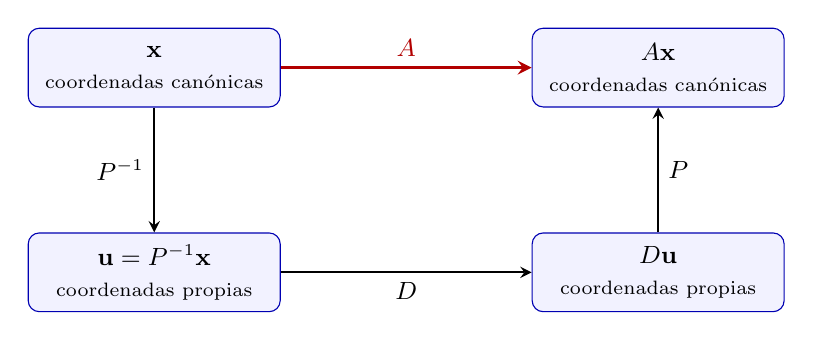
\begin{tikzpicture}[scale=1.0, >=stealth,
  caja/.style={draw=blue!70!black, fill=blue!5, rounded corners, minimum width=3.2cm, minimum height=1cm, align=center}]
\node[caja] (x)  at (0,2.6)   {\small $\mathbf{x}$\\[-1pt] {\scriptsize coordenadas canónicas}};
\node[caja] (Ax) at (6.4,2.6) {\small $A\mathbf{x}$\\[-1pt] {\scriptsize coordenadas canónicas}};
\node[caja] (u)  at (0,0)     {\small $\mathbf{u}=P^{-1}\mathbf{x}$\\[-1pt] {\scriptsize coordenadas propias}};
\node[caja] (Du) at (6.4,0)   {\small $D\mathbf{u}$\\[-1pt] {\scriptsize coordenadas propias}};
\draw[->, red!70!black, very thick] (x) -- node[above] {\small $A$} (Ax);
\draw[->, thick] (x) -- node[left] {\small $P^{-1}$} (u);
\draw[->, thick] (u) -- node[below] {\small $D$} (Du);
\draw[->, thick] (Du) -- node[right] {\small $P$} (Ax);
\end{tikzpicture}
\caption{La diagonalización $A=PDP^{-1}$ como cambio de base. Para aplicar $A$ se puede pasar a coordenadas de vectores propios con $P^{-1}$, escalar cada componente con la matriz diagonal $D$ y volver a coordenadas canónicas con $P$: ambos caminos del diagrama producen el mismo resultado, $A\mathbf{x}=PDP^{-1}\mathbf{x}$.}
\label{fig:diagonalizacion_cajas}
\end{figure}
\begin{theorem} Si $A$ tiene $n$ valores propios distintos, entonces $A$ es diagonalizable.
\begin{proof}
Si $A$ tiene $n$ valores propios distintos, cada multiplicidad algebraica es 1. Como $1 \leq d_i \leq m_i = 1$, entonces $d_i = 1$ para todo $i$, luego $A$ es diagonalizable. Los vectores propios asociados a valores propios distintos son linealmente independientes.
\end{proof}
\end{theorem}


\begin{example}[Diagonalización de una matriz $3\times3$]
Diagonalice la matriz $A=\left(\begin{matrix}
-10 & -71 & -19 \\
3 & 34 & 9 \\
-1 & -61 & -16
\end{matrix}\right).$
\begin{myproof}
\textbf{Paso 1.} Identificamos valores y vectores propios (calculados en el Ejemplo \ref{ex:vvp_multiplicidades}). El polinomio característico $\det(\lambda I - A) = \lambda^3 - 8\lambda^2 + 19\lambda - 12 = 0$ tiene raíces $\lambda_1=1$, $\lambda_2=3$, $\lambda_3=4$ (mult. algebraica 1 c/u), con vectores propios:
\[
v_1 = \begin{pmatrix} \frac{2}{25} \\ -\frac{7}{25} \\ 1 \end{pmatrix}, \quad
v_2 = \begin{pmatrix} \frac{5}{19} \\ -\frac{6}{19} \\ 1 \end{pmatrix}, \quad
v_3 = \begin{pmatrix} \frac{1}{3} \\ -\frac{1}{3} \\ 1 \end{pmatrix}.
\]

\textbf{Paso 2.} Construimos $P$ (columnas = vectores propios) y $D$ (diagonal = valores propios):
\[
P = \begin{pmatrix}
\frac{2}{25} & \frac{5}{19} & \frac{1}{3} \\
-\frac{7}{25} & -\frac{6}{19} & -\frac{1}{3} \\
1 & 1 & 1
\end{pmatrix}, \qquad
D = \begin{pmatrix}
1 & 0 & 0 \\
0 & 3 & 0 \\
0 & 0 & 4
\end{pmatrix}.
\]

\textbf{Paso 3.} Verificamos calculando $P^{-1}$ y el producto $PDP^{-1}$:
\[
P^{-1} = \begin{pmatrix}
-25 & -100 & -25 \\
76 & 361 & 95 \\
-51 & -261 & -69
\end{pmatrix}, \qquad
PDP^{-1} = \begin{pmatrix}
-10 & -71 & -19 \\
3 & 34 & 9 \\
-1 & -61 & -16
\end{pmatrix} = A.
\]
Por lo tanto, $\boxed{A = PDP^{-1}}$ con $P$ y $D$ dadas arriba.
\end{myproof}
\end{example}


\begin{rem}[Cálculo de potencias de una matriz]\label{potdim}
Sea $A$ una matriz diagonalizable, es decir, existe una matriz invertible $P$ y una matriz diagonal $D$ tal que $A = P D P^{-1}$. Entonces, para cualquier entero positivo $k$, se cumple:
\[
A^k = (P D P^{-1})^k = P D^k P^{-1}
\]
Esto se debe a que, al multiplicar $A$ por sí misma $k$ veces, las matrices $P^{-1}P$ se simplifican sucesivamente, resultando en la expresión compacta:
\[
A^k = \underbrace{(P D P^{-1})(P D P^{-1}) \cdots (P D P^{-1})}_{k \text{ veces}} = P D^k P^{-1}
\]
\end{rem}

\begin{example}[Potencia de una matriz usando diagonalización]
Suponga que $(1,1)$ es un vector propio de la matriz $A$ correspondiente al valor propio $3$ y que $(2,1)$ es un vector propio correspondiente al valor propio $-2$. Calcula $A^6 \begin{pmatrix} 4 \\ 3 \end{pmatrix}$.
\begin{myproof}
\textbf{Paso 1.} Establecemos la descomposición $A=PDP^{-1}$ (Observación~\ref{potdim}):
\[
P = \begin{pmatrix} 1 & 2 \\ 1 & 1 \end{pmatrix}, \quad D = \begin{pmatrix} 3 & 0 \\ 0 & -2 \end{pmatrix}, \quad P^{-1} = \begin{pmatrix} -1 & 2 \\ 1 & -1 \end{pmatrix}.
\]

\textbf{Paso 2.} Calculamos $A^6 = PD^6P^{-1}$:
\[
D^6 = \begin{pmatrix} 3^6 & 0 \\ 0 & (-2)^6 \end{pmatrix} = \begin{pmatrix} 729 & 0 \\ 0 & 64 \end{pmatrix},
\]
\begin{align*}
A^6 &= P D^6 P^{-1} =
\begin{pmatrix} 1 & 2 \\ 1 & 1 \end{pmatrix}
\begin{pmatrix} 729 & 0 \\ 0 & 64 \end{pmatrix}
\begin{pmatrix} -1 & 2 \\ 1 & -1 \end{pmatrix}
= \begin{pmatrix} -601 & 1330 \\ -665 & 1394 \end{pmatrix}.
\end{align*}

\textbf{Paso 3.} Aplicamos al vector dado:
\[
A^6 \begin{pmatrix} 4 \\ 3 \end{pmatrix}
= \begin{pmatrix} -601 & 1330 \\ -665 & 1394 \end{pmatrix} \begin{pmatrix} 4 \\ 3 \end{pmatrix}
= \boxed{\begin{pmatrix} 1586 \\ 1522 \end{pmatrix}}.
\]
\end{myproof}
\end{example}


\subsection{La forma canónica de Jordan}\label{subsec:jordan}

Cuando alguna multiplicidad geométrica es menor que la algebraica, la matriz no es diagonalizable: no hay suficientes vectores propios linealmente independientes para formar la matriz $P$. Aun así, toda matriz puede llevarse a una forma «casi diagonal», que es su representación canónica en el caso general.

\begin{definition}[Bloque de Jordan]
Un \textbf{bloque de Jordan} de tamaño $k$ asociado al valor propio $\lambda$ es la matriz $J_k(\lambda)\in M_k(\mathbb{C})$ que tiene $\lambda$ en toda la diagonal, $1$ en la superdiagonal y $0$ en las demás entradas:
\[
J_1(\lambda)=\begin{pmatrix}\lambda\end{pmatrix}, \qquad
J_2(\lambda)=\begin{pmatrix}\lambda & 1\\ 0 & \lambda\end{pmatrix}, \qquad
J_3(\lambda)=\begin{pmatrix}\lambda & 1 & 0\\ 0 & \lambda & 1\\ 0 & 0 & \lambda\end{pmatrix}, \qquad \dots
\]
\end{definition}

\begin{theorem}[Forma canónica de Jordan]\label{thm:cap08:jordan}
Toda matriz $A\in M_n(\mathbb{C})$ es semejante a una matriz formada por bloques de Jordan: existe una matriz invertible $P$ tal que
\[
A = P\, J\, P^{-1}, \qquad
J=\begin{pmatrix} J_{k_1}(\lambda_1) & & \\ & \ddots & \\ & & J_{k_m}(\lambda_m) \end{pmatrix},
\]
donde $\lambda_1,\dots,\lambda_m$ son valores propios de $A$ (posiblemente repetidos entre bloques) y $k_1+\cdots+k_m=n$. La matriz $J$ es única salvo el orden de los bloques, y $A$ es diagonalizable si y solo si todos los bloques son de tamaño $1$.
\end{theorem}

\begin{example}[Forma de Jordan de una matriz no diagonalizable]\label{ex:jordan_2x2}
Encuentre la forma canónica de Jordan de $A=\begin{pmatrix} 1 & 1 \\ -1 & 3 \end{pmatrix}$ y una matriz invertible $P$ tal que $A=PJP^{-1}$.
\begin{myproof}
\textbf{Paso 1.} Calculamos los valores propios: $\det(\lambda I - A) = (\lambda-1)(\lambda-3)+1 = \lambda^2-4\lambda+4 = (\lambda-2)^2$, así que $\lambda=2$ con multiplicidad algebraica $2$.

\textbf{Paso 2.} Calculamos el espacio propio: $A-2I=\begin{pmatrix} -1 & 1 \\ -1 & 1 \end{pmatrix}$, de donde $E_2=\operatorname{gen}\left\{\begin{pmatrix}1\\1\end{pmatrix}\right\}$ y la multiplicidad geométrica es $1<2$: la matriz no es diagonalizable y, por el Teorema \ref{thm:cap08:jordan}, su forma de Jordan es un único bloque $J=J_2(2)=\begin{pmatrix}2&1\\0&2\end{pmatrix}$.

\textbf{Paso 3.} Para construir $P$ tomamos el vector propio $\mathbf{v}_1=\begin{pmatrix}1\\1\end{pmatrix}$ y un \textbf{vector propio generalizado} $\mathbf{v}_2$, solución de $(A-2I)\mathbf{v}_2=\mathbf{v}_1$: el sistema se reduce a $-x+y=1$ y, tomando $x=0$, queda $\mathbf{v}_2=\begin{pmatrix}0\\1\end{pmatrix}$. Con $P=\begin{pmatrix}1&0\\1&1\end{pmatrix}$ (columnas $\mathbf{v}_1$, $\mathbf{v}_2$) se verifica
\[
AP=\begin{pmatrix}2&1\\2&3\end{pmatrix}=PJ.
\]

\textbf{Paso 4.} Como $P$ es invertible, concluimos:
\[
\boxed{A=PJP^{-1} \quad\text{con}\quad J=\begin{pmatrix}2&1\\0&2\end{pmatrix},\quad P=\begin{pmatrix}1&0\\1&1\end{pmatrix}.}
\]
\end{myproof}
\end{example}

\begin{rem}[Alcance y potencias]
La construcción general de la forma de Jordan —cadenas de vectores propios generalizados que determinan el número y el tamaño de los bloques— excede el alcance de este curso; puede consultarse en \cite{hoffman1973algebra}. Para nuestros propósitos basta reconocer la estructura y una consecuencia práctica: igual que con la diagonalización, $A^k=PJ^kP^{-1}$, y las potencias de un bloque de tamaño $2$ tienen forma cerrada:
\[
J_2(\lambda)^k=\begin{pmatrix}\lambda^k & k\,\lambda^{k-1}\\ 0 & \lambda^k\end{pmatrix}.
\]
\end{rem}

\section{Aplicación: sistemas de ecuaciones diferenciales lineales}

\begin{rem}[Alcance de esta sección]
En esta sección se muestra el mecanismo con el que los valores y vectores propios resuelven sistemas lineales de ecuaciones diferenciales: si $A$ es diagonalizable, el cambio de variable $\mathbf{y}=P\mathbf{u}$ desacopla el sistema. El tratamiento sistemático de estos sistemas —valores propios complejos o repetidos, sistemas no homogéneos y aplicaciones adicionales— se desarrolla en el Capítulo~\ref{sistemasedos}.
\end{rem}

\begin{rem}[Solución de ecuaciones diferenciales de primer orden con coeficientes constantes]\label{rem:edo_primer_orden}
Una ecuación diferencial (E.D.) es una igualdad que involucra derivadas y cuya solución consiste en encontrar una función que satisfaga dicha relación. Por ejemplo, para la ecuación $y' = 5y$, la solución se obtiene así:
\[
\frac{dy}{dx} = 5y \implies \int \frac{1}{y} \, dy = \int 5 \, dx \implies \ln|y| = 5x + c \implies y = Ce^{5x}
\]
\textbf{Nota:} El valor de $C$ se determina si se impone una condición inicial (problema de valor inicial, P.V.I.), lo que selecciona una función particular dentro de la familia de soluciones. En general, la solución de $y' = ay$ es $\boxed{y = Ce^{ax}}$.

Por ejemplo, para $y' = 5y$ con $y(0) = 2$, se tiene $y = Ce^{5x}$ y al sustituir $x=0$:
\[
2 = Ce^{0} \implies C = 2
\]
Por lo tanto, la solución particular es $y = 2e^{5x}$.

Este método se puede generalizar a sistemas de ecuaciones diferenciales de primer orden:
\[
\begin{cases}
y_1' = a_{11}y_1 + a_{12}y_2 + \cdots + a_{1n}y_n \\
y_2' = a_{21}y_1 + a_{22}y_2 + \cdots + a_{2n}y_n \\
\hspace{1cm} \vdots \\
y_n' = a_{n1}y_1 + a_{n2}y_2 + \cdots + a_{nn}y_n
\end{cases}
\]
o, en forma matricial:
\[
\begin{pmatrix}
y_1' \\ y_2' \\ \vdots \\ y_n'
\end{pmatrix}
= A
\begin{pmatrix}
y_1 \\ y_2 \\ \vdots \\ y_n
\end{pmatrix}
\]
donde $A$ es la matriz de coeficientes. Si $A$ es diagonalizable, es posible resolver el sistema utilizando los métodos vistos de valores y vectores propios. A continuación se muestra el procedimiento con un ejemplo.
\end{rem}

\begin{example}[Sistema de EDOs: solución por diagonalización]
Resuelve el sistema:
\[
\begin{cases}
y_1' = y_1 + 4y_2 \\
y_2' = 2y_1 + 3y_2
\end{cases}
\]
\begin{myproof}
\textbf{Paso 1.} Escribimos en forma matricial $\mathbf{y}'=A\mathbf{y}$ y diagonalizamos $A = \begin{pmatrix} 1 & 4 \\ 2 & 3 \end{pmatrix}$:
\[
\det(\lambda I - A) = (\lambda-1)(\lambda-3)-8 = \lambda^2-4\lambda-5 = 0 \quad\Rightarrow\quad \lambda_1=5,\ \lambda_2=-1.
\]
Vectores propios: para $\lambda_1=5$, $v_1=\begin{pmatrix}1\\1\end{pmatrix}$; para $\lambda_2=-1$, $v_2=\begin{pmatrix}-2\\1\end{pmatrix}$. Formamos:
\[
P = \begin{pmatrix} 1 & -2 \\ 1 & 1 \end{pmatrix}, \quad D = \begin{pmatrix} 5 & 0 \\ 0 & -1 \end{pmatrix}.
\]

\textbf{Paso 2.} El cambio $\mathbf{y}=P\mathbf{u}$ desacopla el sistema en $\mathbf{u}'=D\mathbf{u}$:
\[
u_1' = 5u_1 \implies u_1 = c_1 e^{5x}, \qquad u_2' = -u_2 \implies u_2 = c_2 e^{-x}.
\]

\textbf{Paso 3.} Regresamos a las variables originales $\mathbf{y}=P\mathbf{u}$:
\[
\begin{pmatrix} y_1 \\ y_2 \end{pmatrix}
= \begin{pmatrix} 1 & -2 \\ 1 & 1 \end{pmatrix} \begin{pmatrix} c_1 e^{5x} \\ c_2 e^{-x} \end{pmatrix}
= \begin{pmatrix} c_1 e^{5x} - 2c_2 e^{-x} \\ c_1 e^{5x} + c_2 e^{-x} \end{pmatrix}.
\]
La solución general es:
\[
\boxed{
\begin{cases}
y_1 = c_1 e^{5x} - 2c_2 e^{-x} \\
y_2 = c_1 e^{5x} + c_2 e^{-x}
\end{cases}
}
\]
\end{myproof}
\end{example}

\begin{theorem}
Si la matriz de coeficientes $A$ de un sistema lineal de ecuaciones diferenciales es diagonalizable, la solución general del sistema
\[
y' = Ay
\]
es
\[
y(x) = c_1 e^{\lambda_1 x} v_1 + \cdots + c_n e^{\lambda_n x} v_n
\]
donde $\lambda_i$ y $v_i$ son los valores y vectores propios de $A$.
\end{theorem}

\begin{proof}
Supongamos que $A$ es diagonalizable, es decir, existe una matriz invertible $P$ y una matriz diagonal $D$ tal que $A = P D P^{-1}$, donde $D = \operatorname{diag}(\lambda_1, \dots, \lambda_n)$.

Consideremos el cambio de variable $y = P u$, donde $u = (u_1, \dots, u_n)^T$. Entonces,
\[
y' = P u'
\]
pero también,
\[
y' = A y = P D P^{-1} y = P D P^{-1} (P u) = P D u
\]
Por lo tanto,
\[
P u' = P D u \implies u' = D u
\]
Como $D$ es diagonal, el sistema $u' = D u$ se desacopla en $n$ ecuaciones independientes:
\[
u_i' = \lambda_i u_i \implies u_i(x) = c_i e^{\lambda_i x}, \quad i = 1, \dots, n
\]
Volviendo a la variable original:
\[
y(x) = P u(x) = c_1 e^{\lambda_1 x} v_1 + \cdots + c_n e^{\lambda_n x} v_n
\]
donde $v_i$ es la $i$-ésima columna de $P$, es decir, el vector propio asociado a $\lambda_i$.

Esto muestra que toda solución es combinación lineal de exponentes de los valores propios multiplicados por sus vectores propios asociados, como se quería demostrar.
\end{proof}


\begin{example}[Problema de valor inicial para un sistema de EDOs]
Resuelve el siguiente problema de valor inicial:
\[
\begin{cases}
y_1' = y_1 + 3y_2 \\
y_2' = 4y_1 + 5y_2
\end{cases}, \quad
\begin{cases}
y_1(0) = 2 \\
y_2(0) = 1
\end{cases}
\]
\begin{myproof}
\textbf{Paso 1.} Diagonalizamos la matriz de coeficientes $A=\begin{pmatrix}1&3\\4&5\end{pmatrix}$:
\[
\det(\lambda I-A) = \lambda^2-6\lambda-7 = (\lambda-7)(\lambda+1) = 0 \quad\Rightarrow\quad \lambda_1=7,\ \lambda_2=-1.
\]
Vectores propios: para $\lambda_1=7$, $v_1=\begin{pmatrix}\frac{1}{2}\\1\end{pmatrix}$; para $\lambda_2=-1$, $v_2=\begin{pmatrix}-\frac{3}{2}\\1\end{pmatrix}$. Formamos:
\[
P = \begin{pmatrix} \tfrac{1}{2} & -\tfrac{3}{2} \\ 1 & 1 \end{pmatrix}, \quad D = \begin{pmatrix} 7 & 0 \\ 0 & -1 \end{pmatrix}.
\]

\textbf{Paso 2.} Con $\mathbf{y}=P\mathbf{u}$ el sistema se desacopla en $u_1'=7u_1$, $u_2'=-u_2$, dando la solución general:
\[
\begin{pmatrix} y_1 \\ y_2 \end{pmatrix}
= P\begin{pmatrix} C_1 e^{7x} \\ C_2 e^{-x} \end{pmatrix}
= \begin{pmatrix} \tfrac{1}{2}C_1 e^{7x} - \tfrac{3}{2}C_2 e^{-x} \\ C_1 e^{7x} + C_2 e^{-x} \end{pmatrix}.
\]

\textbf{Paso 3.} Aplicamos las condiciones iniciales $y_1(0)=2$, $y_2(0)=1$:
\[
\begin{cases}
\tfrac{1}{2}C_1 - \tfrac{3}{2}C_2 = 2 \\
C_1 + C_2 = 1
\end{cases}
\quad\Rightarrow\quad C_1 = \tfrac{7}{4},\quad C_2 = -\tfrac{3}{4}.
\]
La solución particular es:
\[
\boxed{
\begin{cases}
y_1(x) = \dfrac{7}{8} e^{7x} + \dfrac{9}{8} e^{-x} \\[6pt]
y_2(x) = \dfrac{7}{4} e^{7x} - \dfrac{3}{4} e^{-x}
\end{cases}
}
\]
\end{myproof}
\end{example}

\section{El teorema de Cayley-Hamilton}

\begin{theorem}[Cayley-Hamilton]
Sea $A \in M_n(F)$ una matriz cuadrada de orden $n$ sobre un cuerpo $F$. Sea $p_A(\lambda) = \det(\lambda I - A)$ el polinomio característico de $A$. Entonces,
\[
p_A(A) = 0
\]
es decir, toda matriz cuadrada satisface su propia ecuación característica.
\end{theorem}

\begin{proof}
Sea $p_A(\lambda) = \lambda^n + c_{n-1}\lambda^{n-1} + \cdots + c_1\lambda + c_0$ el polinomio característico de $A$. Queremos demostrar que
\[
p_A(A) = A^n + c_{n-1}A^{n-1} + \cdots + c_1A + c_0 I = 0.
\]

Consideremos la matriz $B = \lambda I - A$ y su adjunta $\operatorname{adj}(B)$, que cumple:
\[
B \cdot \operatorname{adj}(B) = \det(B) I = p_A(\lambda) I.
\]
Sustituyendo $\lambda = A$ (es decir, evaluando el polinomio en la matriz $A$), se obtiene:
\[
(AI - A) \cdot \operatorname{adj}(AI - A) = p_A(A) I.
\]
Pero $AI - A = 0$, así que el lado izquierdo es la matriz nula:
\[
0 \cdot \operatorname{adj}(0) = 0 = p_A(A) I.
\]
Por lo tanto,
\[
p_A(A) = 0,
\]
lo que prueba el teorema de Cayley-Hamilton: toda matriz cuadrada anula su propio polinomio característico.
\end{proof}


\section{Valores propios e invertibilidad}

\begin{theorem}[Caracterización de matrices invertibles - Versión 5]
Sea $A$ una matriz $n\times n$, las siguientes afirmaciones son equivalentes: \begin{enumerate}
    \item $A$ es invertible.
    \item La forma escalonada reducida de $A$ es la matriz identidad $I_n$.
    \item $A$ se puede escribir como producto de matrices elementales.
    \item $A$ tiene rango máximo ($\operatorname{rango}(A) = n$).
    \item $\det(A) \neq 0$.
    \item $A\mathbf{x}=\mathbf{0}$ tiene únicamente la solución nula.
    \item $A\mathbf{x}=\mathbf{b}$ es consistente para cualquier vector $\mathbf{b}$.
    \item $A\mathbf{x}=\mathbf{b}$ tiene solución única para cualquier vector $\mathbf{b}$.
    \item Los vectores columna de $A$ son linealmente independientes.
    \item Los vectores fila de $A$ son linealmente independientes.
    \item $\mathcal{C}(A) = \mathbb{R}^n$.
    \item $\mathcal{R}(A) = \mathbb{R}^n$.
    \item $\mathcal{N}(A) = \{\mathbf{0}\}$.
    \item $\mathcal{N}(A^T) = \{\mathbf{0}\}$.
    \item $\dim(\mathcal{C}(A)) = n$.
    \item $\dim(\mathcal{R}(A)) = n$.
    \item $\dim(\mathcal{N}(A)) = 0$.
    \item $\lambda=0$ no es un valor propio de $A.$
\end{enumerate}
\begin{proof}
Las equivalencias entre los ítems 1--17 se establecieron en las versiones anteriores de este teorema. La equivalencia entre el ítem 1 y el ítem 18 es exactamente el Corolario \ref{cor:cerovp}.
\end{proof}
\end{theorem}


\section{Problemas resueltos adicionales}

% --- Valores y vectores propios y multiplicidades ---

% Intermedio

\begin{prob}
Dadas las siguientes matrices calcule sus valores y vectores propios, determine las multiplicidades algebraicas y geométricas correspondientes a cada valor propio. Si la matriz es diagonalizable, calcule su matriz diagonal $D$ asociada.

\begin{enumerate}[$a)$]

\item $A=\left(\begin{matrix}
-3 & 2 \\ 0 & -3
\end{matrix}\right)$

\begin{myproof}
\textbf{Paso 1.} Polinomio característico:
\[
\det(\lambda I - A) = \begin{vmatrix} \lambda+3 & -2 \\ 0 & \lambda+3 \end{vmatrix} = (\lambda+3)^2
\]

\textbf{Paso 2.} Valor propio: $\lambda = -3$ (multiplicidad algebraica 2).

\textbf{Paso 3.} Vectores propios:
\[
(A + 3I)\mathbf{v} = 0 \implies \begin{pmatrix} 0 & 2 \\ 0 & 0 \end{pmatrix} \begin{pmatrix} x \\ y \end{pmatrix} = \begin{pmatrix} 0 \\ 0 \end{pmatrix} \implies 2y=0 \implies y=0
\]
Así, cualquier vector de la forma $\begin{pmatrix} x \\ 0 \end{pmatrix}$ es propio, con $x\neq 0$; la multiplicidad geométrica es 1 (solo un vector propio linealmente independiente).

\textbf{Paso 4.} Como la multiplicidad geométrica es menor que la algebraica,
\[
\boxed{\lambda=-3\ (\text{m.a.}=2,\ \text{m.g.}=1):\ A\ \text{no es diagonalizable}.}
\]
Su forma canónica de Jordan es $J_2(-3)$ (véase la Subsección \ref{subsec:jordan}).
\end{myproof}

\item $A=\left(\begin{matrix}
a & -b \\ b & a
\end{matrix}\right)$

\begin{myproof}
\textbf{Paso 1.} Polinomio característico:
\[
\det(\lambda I - A) = \begin{vmatrix} \lambda-a & b \\ -b & \lambda-a \end{vmatrix} = (\lambda-a)^2 + b^2
\]

\textbf{Paso 2.} Raíces:
\[
\lambda = a \pm ib
\]
Ambos valores propios son complejos conjugados (si $b\neq 0$), de multiplicidad algebraica 1 cada uno.

\textbf{Paso 3.} Para $\lambda_1 = a + ib$:
\[
(A - \lambda_1 I)\mathbf{v} = 0 \implies \begin{pmatrix} a-(a+ib) & -b \\ b & a-(a+ib) \end{pmatrix} = \begin{pmatrix} -ib & -b \\ b & -ib \end{pmatrix}
\]
El vector propio asociado es $\begin{pmatrix} 1 \\ -i \end{pmatrix}$ (o cualquier múltiplo). La multiplicidad geométrica es 1 para cada valor propio.

\textbf{Paso 4.} La matriz es diagonalizable sobre $\mathbb{C}$:
\[
\boxed{D = \begin{pmatrix} a+ib & 0 \\ 0 & a-ib \end{pmatrix}.}
\]
\end{myproof}

\item $A=\left(\begin{matrix}
\cos \theta & -\sen \theta \\ \sen \theta & \cos \theta
\end{matrix}\right),\ 0\leq \theta \leq 2\pi.$

\begin{myproof}
\textbf{Paso 1.} Polinomio característico:
\[
\det(\lambda I - A) = \begin{vmatrix} \lambda-\cos\theta & \sen\theta \\ -\sen\theta & \lambda-\cos\theta \end{vmatrix} = (\lambda-\cos\theta)^2 + \sen^2\theta = \lambda^2 - 2\lambda\cos\theta + 1
\]

\textbf{Paso 2.} Raíces:
\[
\lambda = \cos\theta \pm i\sen\theta = e^{\pm i\theta}
\]
Ambos valores propios son complejos conjugados (salvo $\theta=0,\pi$).

\textbf{Paso 3.} Vectores propios: para $\lambda_1 = e^{i\theta}$, vector propio $\begin{pmatrix} 1 \\ -i \end{pmatrix}$. Multiplicidad algebraica y geométrica: 1 cada una.

\textbf{Paso 4.} La matriz es diagonalizable sobre $\mathbb{C}$:
\[
\boxed{D = \begin{pmatrix} e^{i\theta} & 0 \\ 0 & e^{-i\theta} \end{pmatrix}.}
\]
\end{myproof}

\end{enumerate}
\end{prob}

% Básico
\begin{prob}
Sea $A=\left( \begin{array}{cc} a&-1 \\ 1&4 \end{array} \right)$ donde $a\in \mathbb{R}$ y suponga que $3$ es un valor propio de $A.$ 
\begin{enumerate}[$a)$]
\item Calcule el valor de $a.$
\begin{myproof}
\textbf{Paso 1.} El polinomio característico es:
\[
\det(\lambda I - A) = (\lambda-a)(\lambda-4) + 1 = \lambda^2 - (a+4)\lambda + (4a+1)
\]

\textbf{Paso 2.} Como $\lambda=3$ es valor propio, debe anular el polinomio. Sustituyendo:
\[
3^2 - (a+4)3 + (4a+1) = 0 \implies 9 - 3a - 12 + 4a + 1 = 0 \implies (4a-3a) + (9-12+1) = 0 \implies \boxed{a=2}
\]
\end{myproof}

\item ¿La matriz $A$ tiene valores propios distintos a $3$?
\begin{myproof}
\textbf{Paso 1.} Sustituyendo $a=2$ en el polinomio característico:
\[
\lambda^2 - 6\lambda + (8+1) = \lambda^2 - 6\lambda + 9 = (\lambda-3)^2
\]

\textbf{Paso 2.} Por lo tanto, $\boxed{3\ \text{es el único valor propio (multiplicidad algebraica 2)}}$ y no hay otros valores propios.
\end{myproof}
\end{enumerate}
\end{prob}

% Intermedio
\begin{prob}
Suponga que $A=\left( \begin{array}{ccc} -2&0&1 \\ -5&3&a\\ 4&-2&-1 \end{array} \right)$ donde $a\in \mathbb{R}.$ Encuentre los valores de $a$ de manera que $0, 3, -3$ sean valores propios de $A.$ Calcule los vectores propios asociados a cada valor propio.
\begin{myproof}
\textbf{Paso 1.} El polinomio característico de $A$ es:
\[
p(\lambda) = \det(\lambda I - A) = \lambda^3 + (2a-11)\lambda + (4a-4).
\]

\textbf{Paso 2.} Si los valores propios son $0,3,-3$, entonces $p(\lambda) = \lambda(\lambda-3)(\lambda+3) = \lambda^3 - 9\lambda$. Comparando coeficientes:
\[
4a - 4 = 0 \implies \boxed{a = 1}, \qquad 2(1)-11 = -9\ \checkmark.
\]

\textbf{Paso 3.} Con $a=1$, $A = \begin{pmatrix}-2&0&1\\-5&3&1\\4&-2&-1\end{pmatrix}$. Calculamos los espacios propios.

\textbf{$\lambda=0$:} $(A-0I)\mathbf{v}=0$. Reducción por filas:
\[
A \sim \begin{pmatrix}1&0&-\tfrac{1}{2}\\0&1&-\tfrac{1}{2}\\0&0&0\end{pmatrix}
\]
$x_3$ libre, $x_1=\tfrac{x_3}{2}$, $x_2=\tfrac{x_3}{2}$. Vector propio: $\mathbf{v}_0=\begin{pmatrix}1\\1\\2\end{pmatrix}$.

\textbf{$\lambda=3$:} $(A-3I)\mathbf{v}=0$. $A-3I=\begin{pmatrix}-5&0&1\\-5&0&1\\4&-2&-4\end{pmatrix}$. Reducción:
\[
\sim \begin{pmatrix}1&0&-\tfrac{1}{5}\\0&1&\tfrac{8}{5}\\0&0&0\end{pmatrix}
\]
$x_3$ libre, $x_1=\tfrac{x_3}{5}$, $x_2=-\tfrac{8x_3}{5}$. Vector propio: $\mathbf{v}_3=\begin{pmatrix}1\\-8\\5\end{pmatrix}$.

\textbf{$\lambda=-3$:} $(A+3I)\mathbf{v}=0$. $A+3I=\begin{pmatrix}1&0&1\\-5&6&1\\4&-2&2\end{pmatrix}$. Reducción:
\[
\sim \begin{pmatrix}1&0&1\\0&1&1\\0&0&0\end{pmatrix}
\]
$x_3$ libre, $x_1=-x_3$, $x_2=-x_3$. Vector propio: $\mathbf{v}_{-3}=\begin{pmatrix}1\\1\\-1\end{pmatrix}$.

\textbf{Paso 4.} En resumen, con $a=1$:
\[
\boxed{\mathbf{v}_0=\begin{pmatrix}1\\1\\2\end{pmatrix},\qquad \mathbf{v}_3=\begin{pmatrix}1\\-8\\5\end{pmatrix},\qquad \mathbf{v}_{-3}=\begin{pmatrix}1\\1\\-1\end{pmatrix}.}
\]
\end{myproof}
\end{prob}

% Desafiante
\begin{prob}
Sea $A=\left(\begin{matrix} a&b \\ c&d \end{matrix}\right)$ una matriz de $2\times 2$ y suponga que $b\neq 0.$ Sea $m$ una raíz (real o compleja) de la ecuación $bm^2+(a-d)m-c=0.$  Demuestre que $a+bm$ es un valor propio de $A$ cuyo vector propio asociado es $\begin{pmatrix} 1\\m \end{pmatrix}.$
\begin{myproof}
\textbf{Paso 1.} Sea $\mathbf{v} = \begin{pmatrix} 1 \\ m \end{pmatrix}$. Calculamos:
\[
A\mathbf{v} = \begin{pmatrix} a & b \\ c & d \end{pmatrix} \begin{pmatrix} 1 \\ m \end{pmatrix}
= \begin{pmatrix} a + b m \\ c + d m \end{pmatrix}
\]

\textbf{Paso 2.} Queremos que $A\mathbf{v} = \lambda \mathbf{v}$, es decir,
\[
\begin{cases}
a + b m = \lambda \\
c + d m = \lambda m
\end{cases}
\]
De la primera ecuación, $\lambda = a + b m$. Sustituyendo en la segunda:
\[
c + d m = (a + b m)m \implies c + d m = a m + b m^2 \implies b m^2 + (a - d)m - c = 0
\]

\textbf{Paso 3.} Por hipótesis, $m$ es raíz de esta ecuación, así que ambas condiciones se cumplen: $\lambda = a + b m$ es un valor propio de $A$ con vector propio $\begin{pmatrix} 1 \\ m \end{pmatrix}$, como se quería demostrar.
\end{myproof}
\end{prob}

% --- Diagonalización y potencias ---

% Intermedio
\begin{prob}
Suponga que $\begin{pmatrix} 1 \\ 1 \end{pmatrix}$ es un vector propio de la matriz $A$ correspondiente al valor propio $3$ y que $\begin{pmatrix} 2 \\ 1 \end{pmatrix}$ es un vector propio correspondiente al valor propio $-2$. Calcule $A^{2}\begin{pmatrix} 4 \\ 3 \end{pmatrix}$.
\begin{myproof}
\textbf{Paso 1.} Los vectores propios forman la base de diagonalización. Sea $P = \begin{pmatrix} 1 & 2 \\ 1 & 1 \end{pmatrix}$, $D = \begin{pmatrix} 3 & 0 \\ 0 & -2 \end{pmatrix}$.

\textbf{Paso 2.} Descomponemos $\begin{pmatrix} 4 \\ 3 \end{pmatrix}$ en la base de vectores propios:
\[
P \begin{pmatrix} \alpha \\ \beta \end{pmatrix} = \begin{pmatrix} 4 \\ 3 \end{pmatrix}
\implies
\begin{cases}
\alpha + 2\beta = 4 \\
\alpha + \beta = 3
\end{cases}
\implies \beta = 1, \ \alpha = 2
\]

\textbf{Paso 3.} Aplicamos $A^2 = PD^2P^{-1}$ sobre las coordenadas halladas:
\[
A^2\begin{pmatrix} 4 \\ 3 \end{pmatrix} = P D^2 P^{-1} \begin{pmatrix} 4 \\ 3 \end{pmatrix} = P D^2 \begin{pmatrix} 2 \\ 1 \end{pmatrix} = P \begin{pmatrix} 2\cdot 9 \\ 1\cdot 4 \end{pmatrix} = P \begin{pmatrix} 18 \\ 4 \end{pmatrix}
\]

\textbf{Paso 4.} Calculamos el producto final:
\[
P \begin{pmatrix} 18 \\ 4 \end{pmatrix} = \begin{pmatrix} 1 & 2 \\ 1 & 1 \end{pmatrix} \begin{pmatrix} 18 \\ 4 \end{pmatrix} = \begin{pmatrix} 18 + 8 \\ 18 + 4 \end{pmatrix} \implies \boxed{A^2\begin{pmatrix} 4 \\ 3 \end{pmatrix} = \begin{pmatrix} 26 \\ 22 \end{pmatrix}.}
\]
\end{myproof}
\end{prob}

% Intermedio
\begin{prob}
Sea $A$ una matriz $n\times n$, ya se demostró por inducción sobre $n$ que si $\lambda$ es un valor propio de una matriz $A$ y $v$ es su correspondiente vector propio, entonces $A^{n}{\bf{v}}=\lambda^{n}{\bf{v}}.$  
\begin{enumerate}[$a)$]
\item Suponga que $A=\begin{pmatrix} 1&-14&4 \\ -1&6&-2\\ -2&24&-7
\end{pmatrix}.$ Calcule los valores y vectores propios de $A.$
\begin{myproof}
\textbf{Paso 1.} Calculamos el polinomio característico. Se tiene $\operatorname{tr}(A)=0$, $\det(A)=0$, y la suma de menores principales de orden 2 es $-1$; por tanto:
\[
\det(\lambda I - A) = \lambda^3 - \lambda = \lambda(\lambda-1)(\lambda+1).
\]

\textbf{Paso 2.} Raíces: $\lambda_1=0$, $\lambda_2=1$, $\lambda_3=-1$ (multiplicidad algebraica 1 cada una).

\textbf{Paso 3.} Vectores propios (eliminación gaussiana en $(A-\lambda I)\mathbf{v}=0$):
\begin{itemize}
  \item Para $\lambda=0$: $x_1=-\tfrac{1}{2}x_3$, $x_2=\tfrac{1}{4}x_3$ $\Rightarrow$ $\mathbf{v}_0 = \begin{pmatrix}-2\\1\\4\end{pmatrix}$.
  \item Para $\lambda=1$: $x_1=-\tfrac{4}{7}x_3$, $x_2=\tfrac{2}{7}x_3$ $\Rightarrow$ $\mathbf{v}_1 = \begin{pmatrix}-4\\2\\7\end{pmatrix}$.
  \item Para $\lambda=-1$: $x_1=-\tfrac{3}{5}x_3$, $x_2=\tfrac{1}{5}x_3$ $\Rightarrow$ $\mathbf{v}_{-1} = \begin{pmatrix}-3\\1\\5\end{pmatrix}$.
\end{itemize}
\end{myproof}

\item Sea ${\bf{u}}=\vector(4,-1,7).$ Use el ítem anterior para calcular $A^{20}{\bf{u}}.$
\begin{myproof}
\textbf{Paso 1.} Expresamos $\mathbf{u}=(4,-1,7)^T$ en la base de vectores propios del ítem anterior:
\[
\alpha_0\,\mathbf{v}_0 + \alpha_1\,\mathbf{v}_1 + \alpha_{-1}\,\mathbf{v}_{-1} = \mathbf{u}
\implies \alpha_0=27,\quad \alpha_1=-13,\quad \alpha_{-1}=-2.
\]

\textbf{Paso 2.} Usando $A^n\mathbf{v}=\lambda^n\mathbf{v}$ y que $0^{20}=0$, $1^{20}=1$, $(-1)^{20}=1$:
\[
A^{20}\mathbf{u} = 27\cdot 0^{20}\,\mathbf{v}_0 + (-13)\cdot 1^{20}\,\mathbf{v}_1 + (-2)\cdot(-1)^{20}\,\mathbf{v}_{-1}
= (-13)\begin{pmatrix}-4\\2\\7\end{pmatrix} + (-2)\begin{pmatrix}-3\\1\\5\end{pmatrix}
= \boxed{\begin{pmatrix}58\\-28\\-101\end{pmatrix}}.
\]
\end{myproof}
\end{enumerate}
\end{prob}

 


	


% --- Teorema de Cayley-Hamilton ---

% Intermedio
\begin{prob}
Dada una matriz $A$ de tamaño $n\times n$, se denomina ecuación característica de $A$ a la ecuación
\[
p(\lambda) = \det(\lambda I - A) = 0.
\]
El teorema de Cayley-Hamilton afirma que toda matriz cuadrada $n \times n$ satisface su ecuación característica, es decir, si la ecuación característica de $A$ es $\lambda^n + c_{n-1}\lambda^{n-1} + \cdots + c_0 = 0$, entonces $A^n + c_{n-1}A^{n-1} + \cdots + c_0 I = 0$. En el caso $2 \times 2$, si la ecuación característica es $c_0 + c_1\lambda + \lambda^2 = 0$, entonces $c_0 I + c_1 A + A^2 = 0$.
\begin{enumerate}[$a)$]
\item \textbf{Verifique el teorema de Cayley-Hamilton para la matriz $A = \begin{pmatrix} 3 & 6 \\ 1 & 2 \end{pmatrix}$.}
\begin{myproof}
\textbf{Paso 1.} Calculamos el polinomio característico:
\[
p(\lambda) = \det(\lambda I - A) =
\begin{vmatrix}
\lambda - 3 & -6 \\
-1 & \lambda - 2
\end{vmatrix}
= (\lambda - 3)(\lambda - 2) - 6 = \lambda^2 - 5\lambda
\]
Por lo tanto, $c_1 = -5$ y $c_0 = 0$.

\textbf{Paso 2.} El teorema de Cayley-Hamilton afirma que:
\[
A^2 - 5A = 0 \implies A^2 = 5A
\]

\textbf{Paso 3.} Verificamos calculando ambos lados:
\[
A^2 = \begin{pmatrix} 3 & 6 \\ 1 & 2 \end{pmatrix}^2 = \begin{pmatrix} 3\cdot3 + 6\cdot1 & 3\cdot6 + 6\cdot2 \\ 1\cdot3 + 2\cdot1 & 1\cdot6 + 2\cdot2 \end{pmatrix}
= \begin{pmatrix} 9 + 6 & 18 + 12 \\ 3 + 2 & 6 + 4 \end{pmatrix}
= \begin{pmatrix} 15 & 30 \\ 5 & 10 \end{pmatrix}
\]
\[
5A = 5\begin{pmatrix} 3 & 6 \\ 1 & 2 \end{pmatrix} = \begin{pmatrix} 15 & 30 \\ 5 & 10 \end{pmatrix}
\]

\textbf{Paso 4.} Ambos productos coinciden:
\[
\boxed{A^2 = 5A,}
\]
lo que verifica el teorema de Cayley-Hamilton para esta matriz.
\end{myproof}
\item \textbf{Use diagonalización para calcular $A^3$.}
\begin{myproof}
\textbf{Paso 1.} Los valores propios de $A$ son las raíces de $p(\lambda) = \lambda^2 - 5\lambda = \lambda(\lambda - 5)$, es decir, $\lambda_1 = 5$, $\lambda_2 = 0$.

\textbf{Paso 2.} Los vectores propios asociados son:
\[
\text{Para }\lambda=5: \quad (A - 5I)x = 0 \implies \begin{pmatrix} -2 & 6 \\ 1 & -3 \end{pmatrix} \implies x_1 = 3x_2, \text{ elijo } x_2 = 1 \implies v_1 = \begin{pmatrix} 3 \\ 1 \end{pmatrix}
\]
\[
\text{Para }\lambda=0: \quad (A - 0I)x = 0 \implies \begin{pmatrix} 3 & 6 \\ 1 & 2 \end{pmatrix} \implies x_1 = -2x_2, \text{ elijo } x_2 = 1 \implies v_2 = \begin{pmatrix} -2 \\ 1 \end{pmatrix}
\]
Formamos $P = \begin{pmatrix} 3 & -2 \\ 1 & 1 \end{pmatrix}$ y $D = \begin{pmatrix} 5 & 0 \\ 0 & 0 \end{pmatrix}$.

\textbf{Paso 3.} Calculamos $A^3 = P D^3 P^{-1}$:
\[
D^3 = \begin{pmatrix} 125 & 0 \\ 0 & 0 \end{pmatrix}, \qquad
P^{-1} = \frac{1}{5} \begin{pmatrix} 1 & 2 \\ -1 & 3 \end{pmatrix}
\]
\[
A^3 = \begin{pmatrix} 3 & -2 \\ 1 & 1 \end{pmatrix} \begin{pmatrix} 125 & 0 \\ 0 & 0 \end{pmatrix} \frac{1}{5} \begin{pmatrix} 1 & 2 \\ -1 & 3 \end{pmatrix}
\implies \boxed{A^3 = \begin{pmatrix} 75 & 150 \\ 25 & 50 \end{pmatrix}.}
\]
El literal $d)$ obtiene este mismo resultado mediante el teorema de Cayley-Hamilton.
\end{myproof}
\item \textbf{El teorema de Cayley-Hamilton provee una forma de calcular potencias de una matriz. Demuestre que $A^3 = -c_1A^2 - c_0A$.}
\begin{myproof}
\textbf{Paso 1.} Por el teorema de Cayley-Hamilton, $A^2 + c_1A + c_0I = 0$, así que $A^2 = -c_1A - c_0I$.

\textbf{Paso 2.} Multiplicando ambos lados por $A$:
\[
A^3 = A \cdot A^2 = A(-c_1A - c_0I) = -c_1A^2 - c_0A,
\]
que es la relación pedida.
\end{myproof}
\item \textbf{Use el ítem anterior para calcular $A^3$ con la matriz $A = \begin{pmatrix} 3 & 6 \\ 1 & 2 \end{pmatrix}$. Compare con el resultado obtenido por diagonalización.}
\begin{myproof}
\textbf{Paso 1.} Para esta matriz, $c_1 = -5$, $c_0 = 0$, así que:
\[
A^3 = -(-5)A^2 - 0 \cdot A = 5A^2
\]

\textbf{Paso 2.} Ya calculamos $A^2 = \begin{pmatrix} 15 & 30 \\ 5 & 10 \end{pmatrix}$ en el literal $a)$, así que:
\[
A^3 = 5 \begin{pmatrix} 15 & 30 \\ 5 & 10 \end{pmatrix} \implies \boxed{A^3 = \begin{pmatrix} 75 & 150 \\ 25 & 50 \end{pmatrix},}
\]
que coincide exactamente con el resultado obtenido por diagonalización en el literal $b)$.
\end{myproof}
\end{enumerate}
\end{prob}

% --- Valores propios e invertibilidad ---

% Básico
\begin{prob} Suponga que $A$ es una matriz invertible con valor propio $\lambda$ y su vector propio correspondiente ${\bf{v}}.$ ¿Es  ${\bf{v}}$ un vector propio de $A^{-1}$? Haga una demostración o muestre un contraejemplo.
\begin{myproof}
\textbf{Paso 1.} Como $A$ es invertible, $\lambda \neq 0$ (Corolario \ref{cor:cerovp}), así que $\lambda^{-1}$ existe.

\textbf{Paso 2.} Aplicando $A^{-1}$ a ambos lados de $A\mathbf{v} = \lambda \mathbf{v}$:
\[
A\mathbf{v} = \lambda \mathbf{v} \implies \mathbf{v} = \lambda\, A^{-1} \mathbf{v} \implies A^{-1} \mathbf{v} = \lambda^{-1} \mathbf{v}
\]
Por lo tanto, $\mathbf{v}$ sí es vector propio de $A^{-1}$, con valor propio $\lambda^{-1}$.
\end{myproof}
\end{prob}

% Básico
\begin{prob} Suponga que $A$ es una matriz invertible y ${\bf{v}}$ es uno de sus vectores propios.  ¿Es $3{\bf{v}}$ un vector propio de $A^{-1}$? ¿Cuál será su valor propio correspondiente? Haga una demostración o muestre un contraejemplo.
\begin{myproof}
Sí, porque si $A\mathbf{v} = \lambda \mathbf{v}$, entonces $A^{-1}(3\mathbf{v}) = 3A^{-1}\mathbf{v} = 3\lambda^{-1} \mathbf{v} = \lambda^{-1}(3\mathbf{v})$. Así, $3\mathbf{v}$ es también vector propio de $A^{-1}$ con el mismo valor propio $\lambda^{-1}$.
\end{myproof}
\end{prob}

% --- Sistemas de ecuaciones diferenciales ---

% Intermedio
\begin{prob}
Resuelva los siguientes sistemas de ecuaciones diferenciales usando diagonalización
\begin{enumerate}[$(a)$]
\item $\left\lbrace \begin{matrix}
y_{1}^{\prime}&=&y_1+2y_2\\
y_{2}^{\prime}&=&2y_1+y_2\\
\end{matrix} \right. $ con las condiciones iniciales $y_{1}(0)=3,$ $y_{2}(0)=1.$

\begin{myproof}
\textbf{Paso 1.} La matriz de coeficientes es $A = \begin{pmatrix} 1 & 2 \\ 2 & 1 \end{pmatrix}$, con polinomio característico $\lambda^2 - 2\lambda - 3 = 0 \implies \lambda_1=3, \lambda_2=-1$.

\textbf{Paso 2.} Vectores propios: para $\lambda=3$, $\mathbf{v}_1 = \begin{pmatrix} 1 \\ 1 \end{pmatrix}$; para $\lambda=-1$, $\mathbf{v}_2 = \begin{pmatrix} 1 \\ -1 \end{pmatrix}$.

\textbf{Paso 3.} Solución general:
\[
\mathbf{y}(x) = c_1 e^{3x} \begin{pmatrix} 1 \\ 1 \end{pmatrix} + c_2 e^{-x} \begin{pmatrix} 1 \\ -1 \end{pmatrix}
\]

\textbf{Paso 4.} Condiciones iniciales: $y_1(0)=3$, $y_2(0)=1$ $\implies$ $c_1 + c_2 = 3$, $c_1 - c_2 = 1$ $\implies$ $c_1 = 2$, $c_2 = 1$. Solución particular:
\[
\boxed{y_1(x) = 2e^{3x} + e^{-x},\quad y_2(x) = 2e^{3x} - e^{-x}.}
\]
\end{myproof}

\item $\left\lbrace \begin{matrix}
y_{1}^{\prime}&=&4y_1+y_2\\
y_{2}^{\prime}&=&3y_1+2y_2\\
\end{matrix} \right. $ con las condiciones iniciales $y_{1}(0)=1,$ $y_{2}(0)=5.$

\begin{myproof}
\textbf{Paso 1.} $A = \begin{pmatrix} 4 & 1 \\ 3 & 2 \end{pmatrix}$, con polinomio característico $\lambda^2 - 6\lambda + 5 = 0 \implies \lambda_1=5, \lambda_2=1$.

\textbf{Paso 2.} Vectores propios: para $\lambda=5$, $\mathbf{v}_1 = \begin{pmatrix} 1 \\ 1 \end{pmatrix}$; para $\lambda=1$, $\mathbf{v}_2 = \begin{pmatrix} 1 \\ -3 \end{pmatrix}$.

\textbf{Paso 3.} Solución general:
\[
\mathbf{y}(x) = c_1 e^{5x} \begin{pmatrix} 1 \\ 1 \end{pmatrix} + c_2 e^{x} \begin{pmatrix} 1 \\ -3 \end{pmatrix}
\]

\textbf{Paso 4.} Con las condiciones iniciales $y_1(0)=1$, $y_2(0)=5$:
\[
\begin{cases}
c_1 + c_2 = 1 \\
c_1 - 3c_2 = 5
\end{cases}
\implies c_1 = 2,\ c_2 = -1
\]
Solución particular:
\[
\boxed{y_1(x) = 2e^{5x} - e^{x},\quad y_2(x) = 2e^{5x} + 3e^{x}.}
\]
\end{myproof}

\item $\left\lbrace \begin{matrix}
y_{1}^{\prime}&=&4y_1+y_3\\
y_{2}^{\prime}&=&-2y_1+y_2\\
y_{3}^{\prime}&=&-2y_1+y_3\\
\end{matrix} \right. $ con las condiciones iniciales $y_{1}(0)=-1,$ $y_{2}(0)=1,$ $y_3(0)=0.$

\begin{myproof}
\textbf{Paso 1.} La matriz es $A = \begin{pmatrix} 4 & 0 & 1 \\ -2 & 1 & 0 \\ -2 & 0 & 1 \end{pmatrix}$, con polinomio característico $\det(\lambda I - A) = (\lambda-1)(\lambda-2)(\lambda-3) = 0$: valores propios $\lambda_1=1$, $\lambda_2=2$, $\lambda_3=3$ (multiplicidad algebraica 1 cada uno).

\textbf{Paso 2.} Vectores propios:
\begin{itemize}
  \item $\lambda=1$: $\mathbf{v}_1 = \begin{pmatrix} 0 \\ 1 \\ 0 \end{pmatrix}$; \quad $\lambda=2$: $\mathbf{v}_2 = \begin{pmatrix} -1 \\ 2 \\ 2 \end{pmatrix}$; \quad $\lambda=3$: $\mathbf{v}_3 = \begin{pmatrix} 1 \\ -1 \\ -1 \end{pmatrix}$.
\end{itemize}

\textbf{Paso 3.} Solución general:
\[
\mathbf{y}(x) = c_1 e^{x} \begin{pmatrix} 0 \\ 1 \\ 0 \end{pmatrix} + c_2 e^{2x} \begin{pmatrix} -1 \\ 2 \\ 2 \end{pmatrix} + c_3 e^{3x} \begin{pmatrix} 1 \\ -1 \\ -1 \end{pmatrix}
\]

\textbf{Paso 4.} Condiciones iniciales $y_1(0)=-1$, $y_2(0)=1$, $y_3(0)=0$:
\[
\begin{cases}
-c_2 + c_3 = -1 \\
c_1 + 2c_2 - c_3 = 1 \\
2c_2 - c_3 = 0
\end{cases}
\implies c_1=1,\quad c_2=-1,\quad c_3=-2.
\]
Solución particular:
\[
\boxed{
\begin{cases}
y_1(x) = e^{2x} - 2e^{3x} \\[4pt]
y_2(x) = e^{x} - 2e^{2x} + 2e^{3x} \\[4pt]
y_3(x) = -2e^{2x} + 2e^{3x}
\end{cases}
}
\]
\end{myproof}
\end{enumerate}
\end{prob}


% Desafiante
\begin{prob}
En ocasiones es posible resolver una ecuación diferencial de un grado superior con coeficientes constantes expresándola como un sistema de ecuaciones diferenciales de grado uno. Dada la ecuación diferencial $y^{\prime \prime}-y^{\prime}-6y=0$ demuestre que con las sustituciones $y_{1}=y$ y $y_{2}=y^{\prime}$ se puede construir el sistema
\[
\left\lbrace \begin{matrix}
y_{1}^{\prime}&=& y_2\\
y_{2}^{\prime}&=&6y_1+y_2\\
\end{matrix} \right.
\]
Resuelva este sistema y use sus resultados para resolver la ecuación diferencial original. Realice un procedimiento similar para las ecuaciones $y^{\prime \prime}+y^{\prime}-12y=0$ y $y^{\prime \prime \prime}-6y^{\prime\prime}+11y^{\prime}-6y=0.$
\begin{myproof}
\textbf{Paso 1.} Para $y''-y'-6y=0$, definimos $y_1=y$, $y_2=y'$. Entonces $y_1'=y_2$, $y_2'=y''=y'+6y=y_2+6y_1$, y el sistema es:
\[
\begin{pmatrix} y_1' \\ y_2' \end{pmatrix} = \begin{pmatrix} 0 & 1 \\ 6 & 1 \end{pmatrix} \begin{pmatrix} y_1 \\ y_2 \end{pmatrix}
\]

\textbf{Paso 2.} El polinomio característico es $\lambda^2 - \lambda - 6 = 0 \implies \lambda=3,-2$.

\textbf{Paso 3.} Como $y=y_1$, la solución de la ecuación original es:
\[
\boxed{y(x) = c_1 e^{3x} + c_2 e^{-2x}.}
\]

\textbf{Paso 4.} Repitiendo el procedimiento para las otras ecuaciones:
\begin{itemize}
  \item $y'' + y' - 12y = 0$: sistema $\begin{pmatrix} 0 & 1 \\ 12 & -1 \end{pmatrix}$, raíces $\lambda=3,-4$ $\implies$ $y(x)=c_1e^{3x}+c_2e^{-4x}$.
  \item $y''' - 6y'' + 11y' - 6y = 0$: sistema de $3\times 3$, polinomio característico $\lambda^3 - 6\lambda^2 + 11\lambda - 6 = 0$ (raíces $\lambda=1,2,3$) $\implies$ $y(x)=c_1e^{x}+c_2e^{2x}+c_3e^{3x}$.
\end{itemize}
\end{myproof}
\end{prob}


% Desafiante
\begin{prob}
En la figura se muestra un circuito LRC en paralelo, el cual contiene una resistencia en ohms ($\Omega$), un inductor con inductancia en henries ($H$) y un capacitor con capacitancia en faradios ($F$) . Es posible demostrar en teoría de circuitos que en un tiempo $t$ la corriente $i_{L}$ a través del inductor y el voltaje $v_{C}$ dado por el capacitor son solución del sistema de ecuaciones diferenciales lineales
\[ \begin{pmatrix}
i_{L}^{\prime}(t)\\v_{C}^{\prime}(t)\\
\end{pmatrix} =\begin{pmatrix} 0&\dfrac{1}{L} \\ \dfrac{-1}{C} & \dfrac{-1}{RC}
\end{pmatrix} \begin{pmatrix} i_{L} (t)\\v_{C}(t)  \end{pmatrix} \]
\begin{enumerate}[$(a)$]
\item Calcule la solución general del sistema cuando $R=1\ \Omega,$ $L=1\ H,$ y $C=0.5\ F.$
\begin{myproof}
\textbf{Paso 1.} Con $R=1$, $L=1$ y $C=0.5$ se tiene $\tfrac{1}{L}=1$, $\tfrac{1}{C}=2$ y $\tfrac{1}{RC}=2$, así que la matriz del sistema es $A = \begin{pmatrix} 0 & 1 \\ -2 & -2 \end{pmatrix}$.

\textbf{Paso 2.} Polinomio característico: $\lambda^2 + 2\lambda + 2 = 0 \implies \lambda = -1 \pm i$.

\textbf{Paso 3.} Para $\lambda = -1+i$ un vector propio es $\mathbf{v} = \begin{pmatrix} 1 \\ -1+i \end{pmatrix} = \begin{pmatrix} 1 \\ -1 \end{pmatrix} + i\begin{pmatrix} 0 \\ 1 \end{pmatrix}$. Separando las partes real e imaginaria de $e^{\lambda t}\,\mathbf{v}$ se obtiene la solución general real:
\[
\begin{pmatrix} i_L(t) \\ v_C(t) \end{pmatrix}
= c_1\, e^{-t}\begin{pmatrix} \cos t \\ -\cos t - \sen t \end{pmatrix}
+ c_2\, e^{-t}\begin{pmatrix} \sen t \\ \cos t - \sen t \end{pmatrix},
\]
donde $c_1$ y $c_2$ se determinan por condiciones iniciales.
\end{myproof}

\item Calcule $i_{L}$ y $v_{C}$ cuando $i_{L}(0)=2$ amperios y $v_{C}(0)=1$ voltio.
\begin{myproof}
\textbf{Paso 1.} Evaluando la solución general del literal anterior en $t=0$: $i_L(0) = c_1 = 2$ y $v_C(0) = -c_1 + c_2 = 1$, de donde $c_2 = 3$.

\textbf{Paso 2.} Sustituyendo:
\[
\boxed{i_L(t) = e^{-t}\left(2\cos t + 3\,\sen t\right), \qquad
v_C(t) = e^{-t}\left(\cos t - 5\,\sen t\right).}
\]
\end{myproof}

\item ¿Qué ocurre con la corriente y el voltaje si $t\to \infty$? 
\begin{myproof}
Como la parte exponencial es $e^{-t}$ y las funciones $\cos t$ y $\sen t$ son acotadas, tanto la corriente como el voltaje tienden a cero cuando $t\to\infty$.
\end{myproof}
\end{enumerate}
\end{prob}

% --- Cadenas de Markov ---
\section{Algunas aplicaciones adicionales}

Algunas aplicaciones adicionales de los valores y vectores propios se enuncian a continuación:

\begin{definition}
Una \textbf{cadena de Markov} es un proceso estocástico con un número finito de estados, en el cual la probabilidad de transición al siguiente estado depende únicamente del estado actual, y no de los anteriores. Las probabilidades de transición permanecen constantes en el tiempo.
\end{definition}

\begin{theorem}
Sea $P$ la matriz de transición de una cadena de Markov y $x_0$ el vector de probabilidades inicial. Entonces, el vector de probabilidades después de $k$ pasos es
\[
x_k = P^k x_0.
\]
\end{theorem}

\begin{definition}
Un \textbf{vector estacionario} $x$ es un vector de probabilidad tal que $Px = x$, es decir, es un vector propio de $P$ asociado al valor propio $1$, cuyas entradas son no negativas y suman $1$.
\end{definition}

\begin{example}[Cadena de Markov: tres ciudades]
Supón tres ciudades: Boston, Chicago y Los Ángeles. La matriz de transición es
\[
P = \begin{pmatrix}
0.5 & 0.5 & 0 \\
0.5 & 0 & 0.5 \\
0 & 0.5 & 0.5
\end{pmatrix}
\]
y el vector inicial es $x_0 = (100,\, 200,\, 300)^T$. La distribución después de un mes es $x_1 = P x_0$, y después de dos meses $x_2 = P^2 x_0$.
\end{example}


\begin{definition}
Una \textbf{forma cuadrática} en $\mathbb{R}^n$ es una función $Q:\mathbb{R}^n \to \mathbb{R}$ de la forma
\[
Q(x) = x^T A x
\]
donde $A$ es una matriz cuadrada simétrica de orden $n$.
\end{definition}

\begin{theorem}
Sea $Q(x) = x^T A x$ una forma cuadrática y sean $\lambda_1, \dots, \lambda_n$ los valores propios de $A$:
\begin{itemize}
    \item $Q$ es \textbf{definida positiva} si todos los $\lambda_i > 0$.
    \item $Q$ es \textbf{definida negativa} si todos los $\lambda_i < 0$.
    \item $Q$ es \textbf{indefinida} si existen $\lambda_i > 0$ y $\lambda_j < 0$.
\end{itemize}
\end{theorem}

\begin{example}[Forma cuadrática definida positiva]
Sea $A = \begin{pmatrix} 2 & 0 \\ 0 & 3 \end{pmatrix}$. Entonces,
\[
Q(x, y) = \begin{pmatrix} x & y \end{pmatrix}
\begin{pmatrix} 2 & 0 \\ 0 & 3 \end{pmatrix}
\begin{pmatrix} x \\ y \end{pmatrix}
= 2x^2 + 3y^2
\]
Como ambos valores propios son positivos, $Q$ es definida positiva.
\end{example}

\begin{definition}
Un \textbf{sistema dinámico} es un sistema cuyo estado evoluciona con el tiempo según una regla de evolución. Formalmente, es una tupla $(T, X, \Phi)$ donde $T$ es el conjunto de tiempos, $X$ es el espacio de estados y $\Phi: U \subseteq (T \times X) \to X$ es la función de evolución que cumple:
\begin{align*}
\Phi(0, x) &= x \\
\Phi(t_2, \Phi(t_1, x)) &= \Phi(t_2 + t_1, x)
\end{align*}
para los valores de $t_1, t_2$ y $x$ donde esté definida.
\end{definition}

\begin{example}[Sistema dinámico discreto: ecuación logística]
\textbf{Sistema dinámico discreto:} La ecuación logística discreta
\[
x_{t+1} = a x_t (1 - x_t)
\]
modela la evolución de una población con efecto de saturación.
\end{example}

\begin{example}[Sistema dinámico continuo: crecimiento logístico]
\textbf{Sistema dinámico continuo:} La ecuación diferencial
\[
\frac{dx}{dt} = a x (1 - x)
\]
describe el crecimiento poblacional continuo con límite superior.
\end{example}

\begin{theorem}
\textbf{(Principio de superposición para sistemas lineales)}\\
Si $x_1(t)$ y $x_2(t)$ son soluciones de un sistema dinámico lineal homogéneo, entonces cualquier combinación lineal $c_1 x_1(t) + c_2 x_2(t)$ también es solución.
\end{theorem}

\section{Problemas propuestos}

% --- Valores y vectores propios y multiplicidades ---

% Básico
\begin{prob}
Calcule los valores y vectores propios de $A=\begin{pmatrix} 5 & 4 \\ 1 & 2 \end{pmatrix}$.
\end{prob}

% Básico
\begin{prob}
Sin calcular el polinomio característico, dé los valores propios de la matriz triangular
$A=\begin{pmatrix} 3 & 1 & -2 \\ 0 & -1 & 4 \\ 0 & 0 & 3 \end{pmatrix}$
y determine sus multiplicidades algebraicas.
\end{prob}

% Básico
\begin{prob}
Verifique que $\mathbf{v}=\begin{pmatrix} 1 \\ 2 \end{pmatrix}$ es un vector propio de $A=\begin{pmatrix} 4 & 1 \\ 2 & 5 \end{pmatrix}$ y encuentre su valor propio asociado.
\end{prob}

% Intermedio
\begin{prob}
Calcule los valores propios, los vectores propios y las multiplicidades algebraicas y geométricas de
$A=\begin{pmatrix} 2 & 1 & 0 \\ 0 & 2 & 0 \\ 0 & 0 & 3 \end{pmatrix}$.
¿Es $A$ diagonalizable?
\end{prob}

% Intermedio
\begin{prob}
Encuentre el valor de $a$ para que $\lambda=2$ sea un valor propio de $A=\begin{pmatrix} 1 & a \\ 2 & 1 \end{pmatrix}$. Con ese valor de $a$, calcule el otro valor propio de $A$.
\end{prob}

% --- Diagonalización y potencias ---

% Básico
\begin{prob}
Sea $D=\begin{pmatrix} 2 & 0 \\ 0 & -3 \end{pmatrix}$. Calcule $D^{5}$ y explique por qué los valores propios de $D^{5}$ son los de $D$ elevados a la quinta potencia.
\end{prob}

% Intermedio
\begin{prob}
Diagonalice la matriz $A=\begin{pmatrix} 1 & 3 \\ 2 & 2 \end{pmatrix}$: encuentre una matriz invertible $P$ y una matriz diagonal $D$ tales que $A=PDP^{-1}$, y verifique que $AP=PD$.
\end{prob}

% Intermedio
\begin{prob}
Sabiendo que $\begin{pmatrix} 1 \\ 1 \end{pmatrix}$ y $\begin{pmatrix} 1 \\ -1 \end{pmatrix}$ son vectores propios de $A=\begin{pmatrix} 3 & 2 \\ 2 & 3 \end{pmatrix}$, calcule $A^{4}\begin{pmatrix} 3 \\ 1 \end{pmatrix}$ sin calcular la matriz $A^{4}$.
\end{prob}

% Desafiante
\begin{prob}
Sea $A$ una matriz de $2\times 2$ con valores propios $\lambda_1$ y $\lambda_2$. Demuestre que $\operatorname{tr}(A)=\lambda_1+\lambda_2$ y que $\det(A)=\lambda_1\lambda_2$.
\end{prob}

% Desafiante
\begin{prob}
Sea $A=\begin{pmatrix} a & b \\ b & c \end{pmatrix}$ una matriz simétrica con entradas reales. Demuestre que sus valores propios son reales y que, si $\lambda_1\neq\lambda_2$, los vectores propios asociados son ortogonales.
\end{prob}

% --- Teorema de Cayley-Hamilton e invertibilidad ---

% Intermedio
\begin{prob}
Verifique el teorema de Cayley-Hamilton para $A=\begin{pmatrix} 2 & 1 \\ 1 & 3 \end{pmatrix}$ y úselo para expresar $A^{-1}$ como un polinomio en $A$.
\end{prob}

% Intermedio
\begin{prob}
Demuestre que si $\lambda$ es un valor propio de $A$ con vector propio $\mathbf{v}$, entonces $\lambda+c$ es un valor propio de $A+cI$ con el mismo vector propio. Use este resultado para hallar los valores propios de $A+3I$ sabiendo que los de $A$ son $1$ y $-2$.
\end{prob}

% Desafiante
\begin{prob}
Demuestre que si $A^{2}=A$ (matriz idempotente), entonces sus valores propios solo pueden ser $0$ o $1$; y que si $A^{k}=0$ para algún entero positivo $k$ (matriz nilpotente), entonces su único valor propio es $0$.
\end{prob}

% --- Aplicaciones ---

% Básico
\begin{prob}
Para la matriz de transición $P=\begin{pmatrix} 0.8 & 0.3 \\ 0.2 & 0.7 \end{pmatrix}$ de una cadena de Markov, encuentre el vector estacionario, es decir, el vector propio asociado a $\lambda=1$ cuyas entradas son no negativas y suman $1$.
\end{prob}

% Intermedio
\begin{prob}
Resuelva el sistema de ecuaciones diferenciales
\[
\left\lbrace \begin{matrix}
y_{1}^{\prime}&=&2y_1+y_2\\
y_{2}^{\prime}&=&y_1+2y_2\\
\end{matrix} \right.
\]
con las condiciones iniciales $y_{1}(0)=1,$ $y_{2}(0)=3,$ usando diagonalización.
\end{prob}

% Intermedio
\begin{prob}
Clasifique la forma cuadrática $Q(x,y)=3x^{2}+2xy+3y^{2}$ (definida positiva, definida negativa o indefinida) calculando los valores propios de su matriz simétrica asociada.
\end{prob}
